\documentclass[9pt]{IEEEtran}

\usepackage[english]{babel}
\usepackage{graphicx}
\usepackage{epstopdf}
\usepackage{fancyhdr}
\usepackage{amsmath}
\usepackage{amsthm}
\usepackage{amssymb}
\usepackage{url}
\usepackage{array}
\usepackage{textcomp}
\usepackage{listings}
\usepackage{hyperref}
\usepackage{xcolor}
\usepackage{colortbl}
\usepackage{float}
\usepackage{gensymb}
\usepackage{longtable}
\usepackage{supertabular}
\usepackage{multicol}
\usepackage[justification=centering]{caption}
\usepackage{amsmath}
\usepackage{subcaption}

\usepackage[utf8x]{inputenc}

\usepackage[T1]{fontenc}
\usepackage{lmodern}
\input{glyphtounicode}
\pdfgentounicode=1

\graphicspath{{./figures/}}
\DeclareGraphicsExtensions{.pdf,.png,.jpg,.eps}

% correct bad hyphenation here
\hyphenation{op-tical net-works semi-conduc-tor trig-gs}

% ============================================================================================

\title{\vspace{0ex}Logistic Regression}

\author{Aljaž Konec, 63190019\vspace{-4.0ex}}
\date{}
% ============================================================================================

\begin{document}

\maketitle

\section{Introduction}

Logistic regression is one of the most widely used machine learning algorithms for binary classification.
Its use can also be expanded to work on multi-class and ordinal classification problems.
Multi-class regression, also known as known as multinomial logistic regression, extends binary classification to alow for $K$ classes to be predicted.
Ordinal regression, on the other hand, is used when the classes have a natural, clear order to them.
Some such examples may include grades in school, customer satisfaction and modeling of human levels of preference (a scale from, say, 1-5 for "very poor" through "excellent").
In this report we first showcase the implementation details of multinomial logistic regression as well as ordinal logistic regression.
The next section describes how the coeficients of multinomial regression are related to the target classes.
In the final section we showcase an example of a data generating process that is better modeled for ordinal regression than for multinomial regression.


\section{Model implementation}

\subsection*{Multinomial logistic regression}
The multinomial logistic regression model differs from the binary logistic regression model in that it has $K$ sets of coefficients, one for each class.
To calculate the probability of a sample belonging to a certain class, we use the softmax function:
\begin{equation}
    P(y = k | x) = \frac{e^{\beta_k^T x}}{1 + \sum_{j=1}^{K} e^{\beta_j^T x}}
\end{equation}
where $\beta_k$ is the set of coefficients for class $k$.
The loss functions is then defined as the negative log-likelihood over all samples:
\begin{equation}
    -logL(\beta) = -\sum_{i=1}^{N} \sum_{k=1}^{K} \delta_{ik} \log P(y = k | x_i)
\end{equation}
where $\delta_{ik}$ is the indicator function that is 1 if $y_i = k$ and 0 otherwise.
To account for the intercept term, we add a column of ones to the input matrix $X$.
We also add L2 regularization to the loss function.
The resulting $\beta$ is then a matrix of shape $(K, M)$ where $M$ is the number of features in the input matrix $X$.
For predicting the class of a sample, we simply take the class with the highest probability for that sample.

\subsection*{Ordinal logistic regression}

Ordinal logistic regression is a generalization of binary logistic regression to multiple classes that have a natural order to them.
We train $K-2$ thresholds $\tau$ that separate the classes.
These thresholds have to be ordered, i.e. $\tau_1 < \tau_2 < \ldots < \tau_{K-2}$.
We achieve this by appending $\Delta_{k-1}$ to the vector of coefficients $\beta$ for each threshold $\tau_k$.
And defining $\tau_0 = -\infty \leq \tau_1 = 0 \leq \tau_2 = \tau_1 + \Delta_1 \leq \ldots \leq \tau_{K-1} = \tau_{K-2} + \Delta_{K-2} \leq \tau_K = \infty$.
The probability vector of size $K$ is then defined (compontent-wise) as:
\begin{equation*}
    \begin{aligned}
        P(y = k | x) &= P(y <= k-1 | x) - P(y <= k | x)\\
         &= \frac{1}{1 + e^{\tau_k - \beta_k^T x}} - \frac{1}{1 + e^{\tau_{k-1} - \beta_k^T x}}
    \end{aligned}
\end{equation*}
Calculating the loss function is done in a similar way as for multinomial regression, but with the probability vectors defined above.
The resulting $\beta$ is then a matrix of shape $(K-1, M)$ where $M$ is the number of features in the input matrix $X$.

\section{Interpretation of coefficients}
To better understand the coefficients of the multinomial logistic regression model we train a classification model on A dataset of Baskeball Shot Types \cite{basket}.
The dataset contains 8 features: Shot Type, Competition, Player Type, Transition, TwoLegged, Movement, Angle and Distance.
The target variable is the Shot Type, which has 6 classes: Above Head, Dunk, Hook Shot, Layup, Tip-in and Other.
Competition, Player Type and Movement are categorical features that were one-hot encoded.
All features were then centered and scaled appropriately.
This resulted in 12 features and one target variable.

Since coeficients are an estimate they contain some uncertainty.
To model this uncertainty we use 100 repetitions of bootstrapping.
The results are shown in Figure \ref{fig:coef}.
\begin{figure}
    \centering
    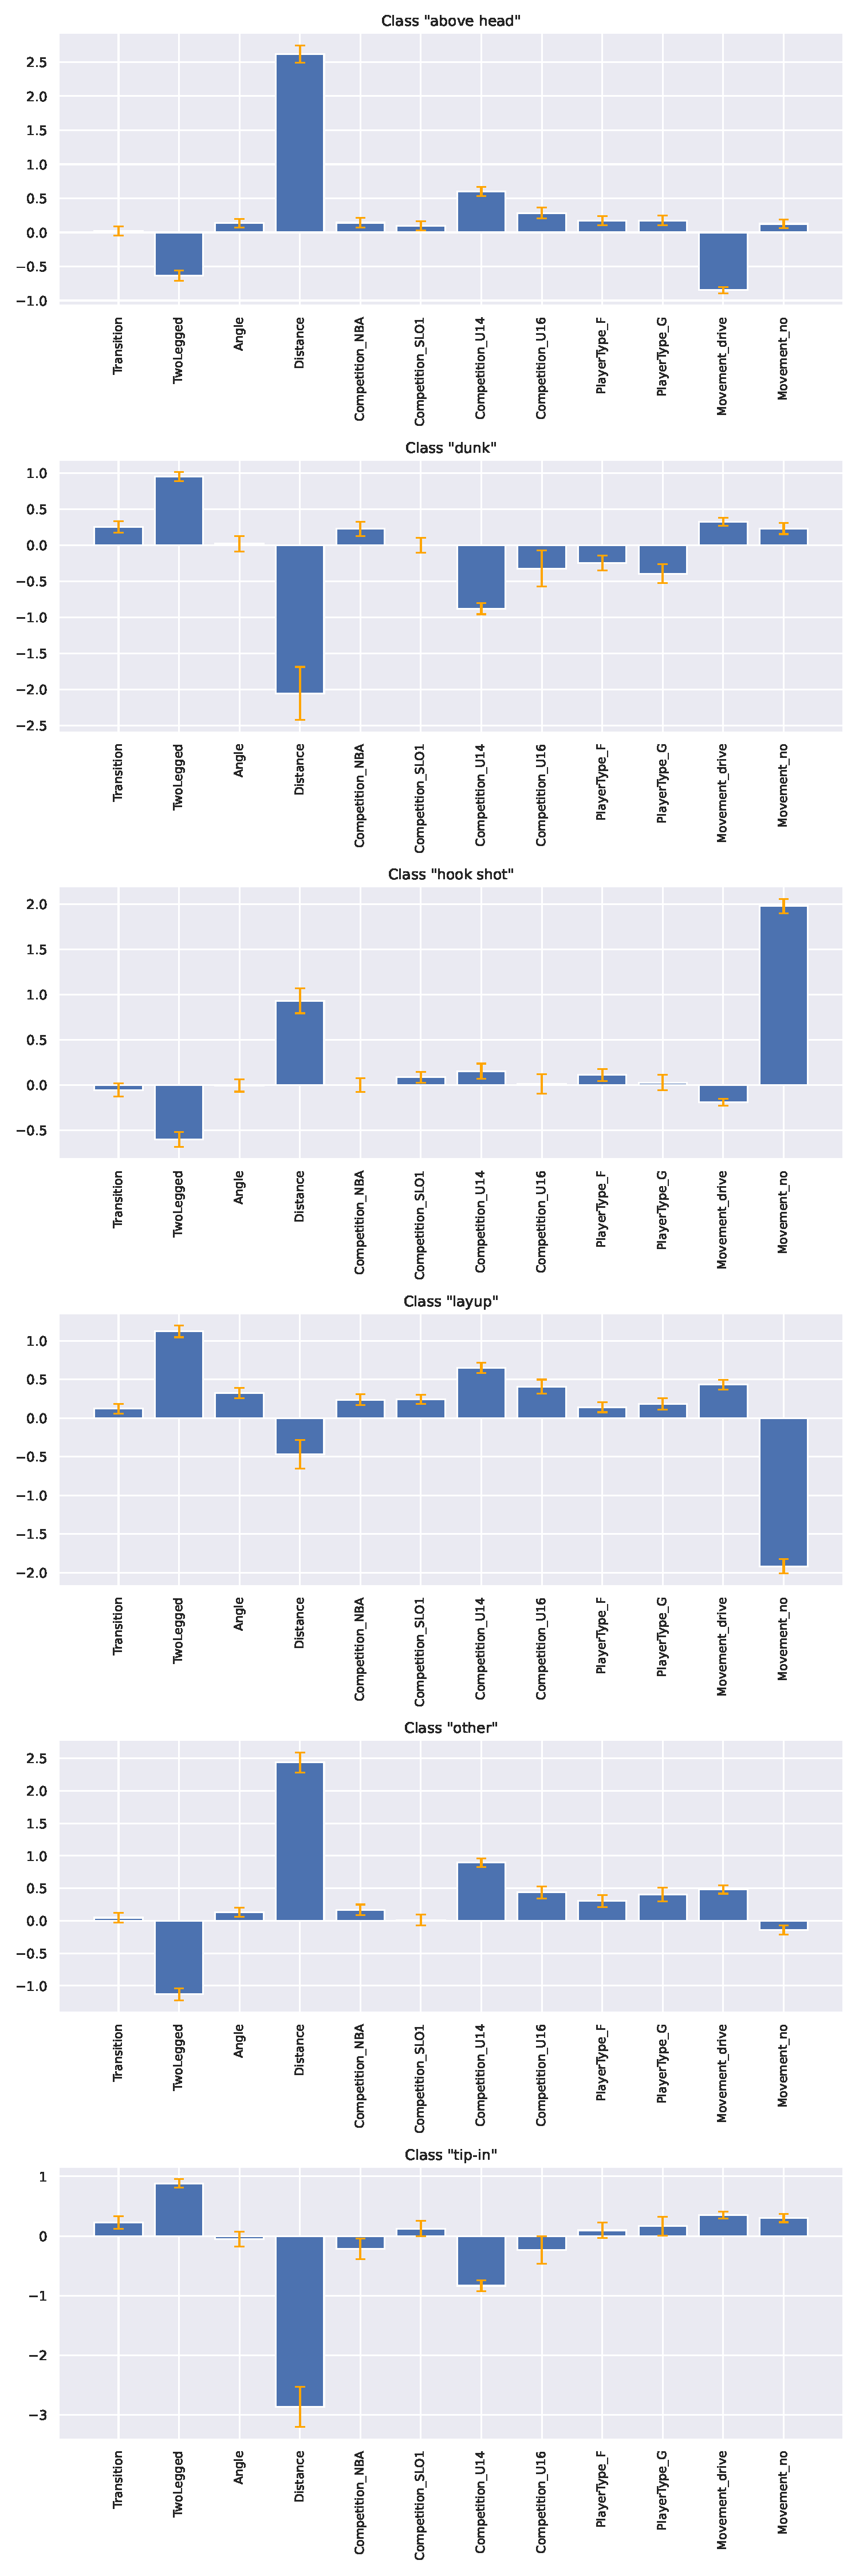
\includegraphics[width=0.4\textwidth]{coefficients.pdf}
    \caption{Coefficients of the multinomial logistic regression model.}
    \label{fig:coef}
\end{figure}
A positive coefficient means that the feature is positively correlated with the class


\section{Conclusion}

A sentence or two to conclude the report. Write when the method works well and what its limitations.

\bibliographystyle{IEEEtran}
\bibliography{main}

\end{document}
